\documentclass[a4paper,11pt,twoside]{article}
%\documentclass[a4paper,11pt,twoside,se]{article}

\usepackage{UmUStudentReport}
\usepackage{verbatim}   % Multi-line comments using \begin{comment}
\usepackage{courier}    % Nicer fonts are used. (not necessary)
\usepackage{pslatex}    % Also nicer fonts. (not necessary)
\usepackage[pdftex]{graphicx}   % allows including pdf figures
\usepackage{listings}
\usepackage{pgf-umlcd}
%\usepackage{lmodern}   % Optional fonts. (not necessary)
%\usepackage{tabularx}
%\usepackage{microtype} % Provides some typographic improvements over default settings
%\usepackage{placeins}  % For aligning images with \FloatBarrier
%\usepackage{booktabs}  % For nice-looking tables
%\usepackage{titlesec}  % More granular control of sections.

% DOCUMENT INFO
% =============
\department{Department of Computing Science}
\coursename{Object-Oriented Programming Methodology 7.5 p}
\coursecode{5DV133}
\title{OU4 Sensor Network}
\author{Johan Eklund ({\tt{kv03jed@cs.umu.se}}) \\ 
Tommie Lindberg ({\tt{c15tlg@cs.umu.se}}) \\
Jakob Lundin ({\tt{c14jln@cs.umu.se}}) \\
Lorenz Gerber ({\tt{dv15lgr@cs.umu.se}}, {\tt{lozger03@student.umu.se}})
}
\date{2016-05-23}
%\revisiondate{2016-01-18}
\instructor{Anders Broberg \\ Niklas Fries \\ Adam Dahlgren \\
  Jonathan Westin \\ Erik Moström \\ Alexander Sutherland}


% DOCUMENT SETTINGS
% =================
\bibliographystyle{plain}
%\bibliographystyle{ieee}
\pagestyle{fancy}
\raggedbottom
\setcounter{secnumdepth}{2}
\setcounter{tocdepth}{2}
%\graphicspath{{images/}}   %Path for images

\usepackage{float}
\floatstyle{ruled}
\newfloat{listing}{thp}{lop}
\floatname{listing}{Listing}



% DEFINES
% =======
%\newcommand{\mycommand}{<latex code>}

% DOCUMENT
% ========
\begin{document}
\lstset{language=C}
\maketitle
\thispagestyle{empty}
\newpage
\tableofcontents
\thispagestyle{empty}
\newpage

\clearpage
\pagenumbering{arabic}

\section{Introduction} 
The assignment was described on the course homepage
\cite{sensornetwork}. The main aim idea was to develop software that
allows to perform experiments on sensor networks as described in
Braginsky and Estrin \cite{braginsky2002}. The main topic of
\cite{braginsky2002} is the use of \textit{rumour routing} as an
energy saving message transportation algorithm that for example
be used in environment surveillance networks.

\section{Compiling and Running of the Program}

\subsection{Javadoc}

\subsection{Specific Design Decisions}

\section{Description of Program Structure}

Figure \ref{fig:uml} shows the UML diagram of the chosen design. 
\begin{figure}
\centering
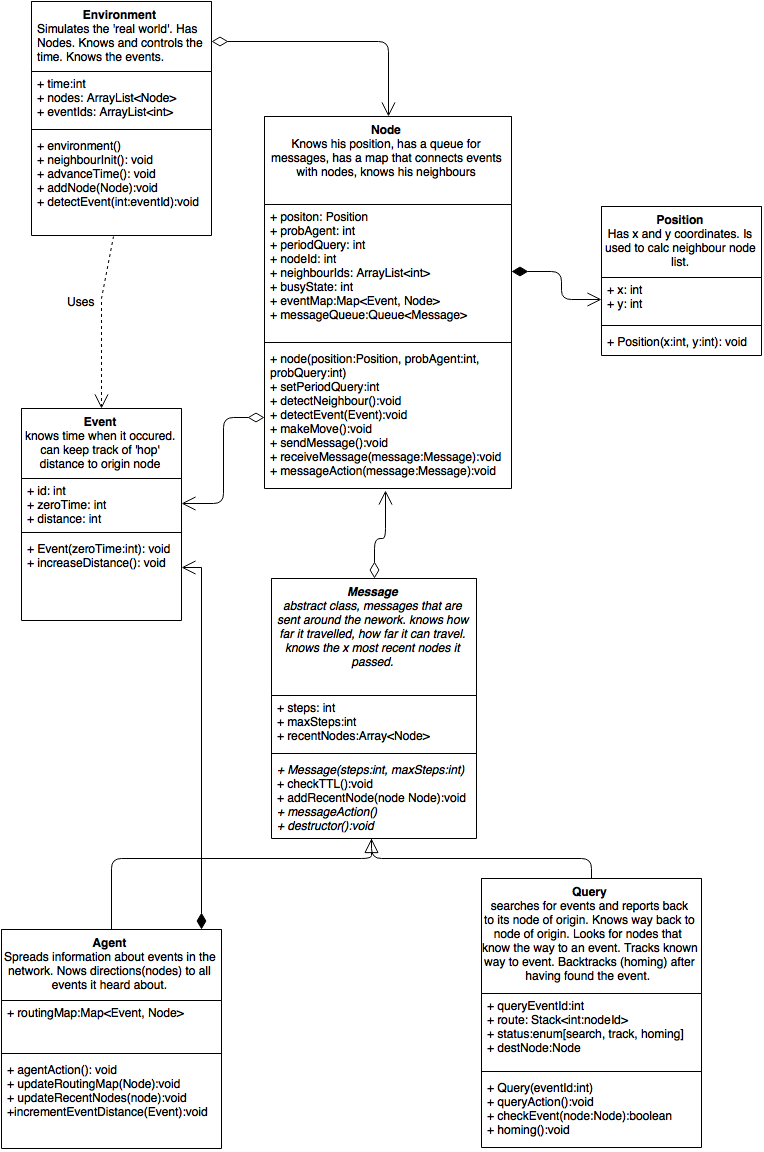
\includegraphics[width=\textwidth]{uml.png}
\caption{\textit{UML diagram for implementing a sensory network application
  that allows testing of the rumour routing algoritm.}}
\label{fig:uml}
\end{figure}



\section{Limitations and Future Development}

\section{Testing Framework}


\section{Individual Contributions}
\subsection{Johan Eklund}
\subsection{Tommie Lindberg}
\subsection{Jakob Lundin}
\subsection{Lorenz Gerber}

\addcontentsline{toc}{section}{\refname}
\bibliography{references}

\end{document}
 
